\chapter{Background}
\label{chap:background}
Al fine di fornire le conoscenze necessarie alla comprensione od eventuale continuazione del lavoro svolto in questo elaborato, risulta necessario introdurre gli argomenti che si andranno ad affrontare durante la tesi, partendo dai dispositivi FPGA.
\section{Field Programmable Gate Array}
\label{FPGA}
Sin dal invenzione dei computer, la loro progrettazione è avvenuta con una rapida evoluzione. A metà degli anni '80, un tipo di architettura diverso da quello convenzionale fu sviluppato, le Field Programmable Gate Array (FPGA). Esse furono costruite tramite un interconnessione effettuata dal progettista tra ROM/PROM o array di porte NAND.
Le FPGA moderne, sono una soluzione prefabbricata, elettronicamente programmabile, atte alla progettazione di sistemi digitali ad alte prestazioni per basso volume. Le FPGA vengono progettate su CAD appositi, come ad esempio VIVADO, senza la necessità di dover modificare la struttura fisicamente.\clearpage
\begin{figure}[h]
\centering
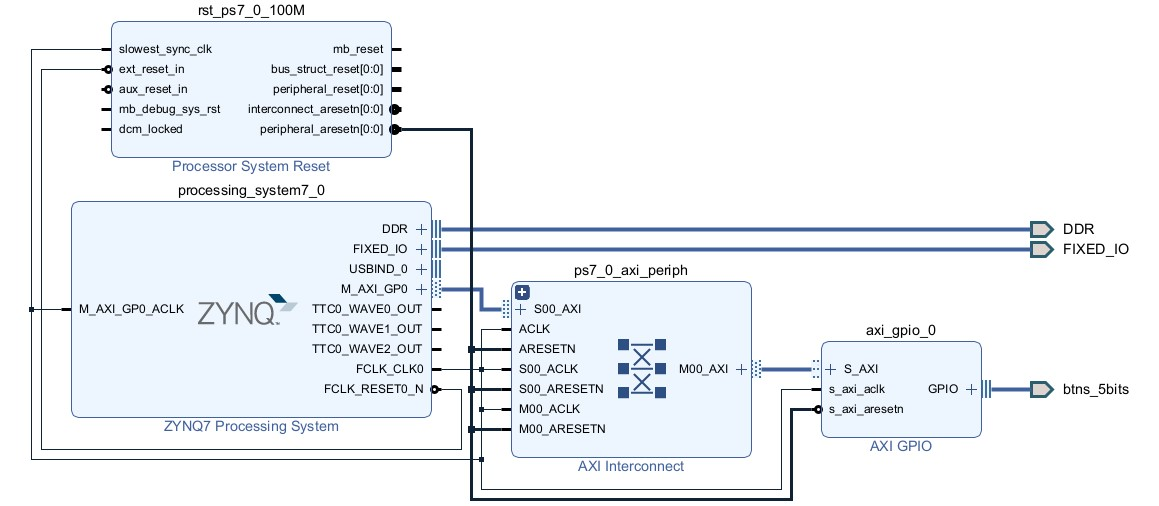
\includegraphics[width=0.8\textwidth]{images/Vivado.jpg}
\caption{Foto di una prototipazione tramite vivado di una FPGA zynq-7000 che sfrutta il GPIO}
\label{VIVADO1}
\end{figure}
Questa famiglia di dispositivi dev'essere immaginataa come un insieme di componenti logici, tali Configurable Logic Block (CLB), come già detto possono essser modificati dal progettista, i CLB sono composti da Look Up Table (LUT), Full Adders, Registi, Multiplexer e funzioni date dall'implementazioni.
Questa divisione in blocchi permette di creare dei cluster interconnessi, rendendo cosi possibile la sintetizzazione di tutte le possibili operazioni booleane e la realizzazione di sistemi complessi. 
\begin{figure}[h]
\centering
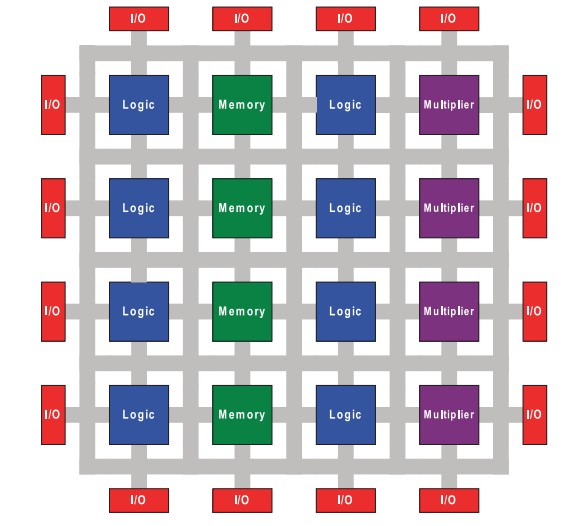
\includegraphics[width=0.3\textwidth]{images/FPGA.jpg}
\caption{Tipica rappresentazione di un FPGA \cite{8187326}}
\end{figure}\\
Le FPGA per loro natura devono comunicare in qualche modo con altri dispositivi, tale comunicazione è gestita da blocchi detti Input Output Block(IOB), essi garantiscono l'interfacciamento tra le risorse della programmable logic (PL) ed il mondo esterno, ogni IOB gestisce un segnale d'input/output ed è in grado di effettuare una conversione, programmabile, tra formati seriali e paralleli, oltre alla gestione di vari standard di I/O e l'eventuale configurazione di Pull-up/Pull-down interni.\\
Data la sempre più crescente quantità di CLB si può pensare come sia necessario aumentare sempre di più l'area di silicio occupata, ma essa è solitamente occupata dai sistemi di interconnessione interna.\\
Le FPGA essendo completamente riprogrammabili possono accogliere dei cores custom, detti Intellectual Property Cores, essi rappresentano dei dispositivi pre-realizzati al fine di compiere una ben precisa azione, essi possono passare da un banale moltiplicatore ad un softcore arm.
\begin{figure}[h]
\centering
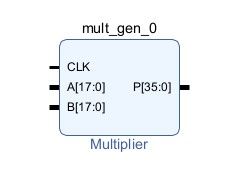
\includegraphics[width=0.3\textwidth]{images/IPcores.jpg}
\caption{Rappresentazione grafica di un IPCore in Vivado}
\end{figure}\\
\subsection{Le FPGA SoC}
L'evoluzione dei processi tecnologici ha portato alla nascita di nuovi tipi di FPGA, le FPGA SoC, esse sono architetture che presentano una interconnessione tra Processore, solitamente della famiglia ARM, ed un FPGA in un unico dispositivo.\clearpage
\begin{figure}[h]
\centering
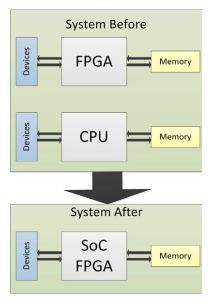
\includegraphics[width=0.4\textwidth]{images/Capture1.png}
\caption{Cambio di paradigma con l'introduzione delle FPGA SoC}
\end{figure}
La loro fusione permette una maggior integrazione, anche lato connettività e quindi Cloud, un minor consumo ed una comunicazione molto più efficiente tra i due grazie ad una larghezza di banda superiore ed una latenza nettamente inferiore a prima.
\begin{figure}[h]
\centering
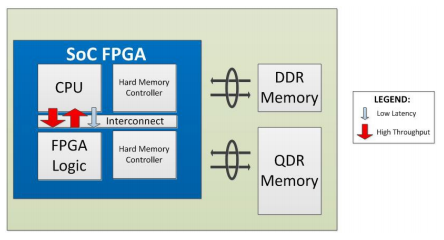
\includegraphics[width=0.6\textwidth]{images/Capture8.png}
\caption{Schema rappresentativo FPGA SoC}
\end{figure}\\
\subsection{Architettura Zynq-7000}
L'architettura Zynq-7000 è basata sul architettura Xilinx All Programmable System On Chip (AP SoC). I dispositivi di questa famiglia sono formati da un dual-single Core ARM Cortex A9 su cui si basa il Processing System (PS), includendo anche una on-chip memory, interfacce con memorie esterne e le periferiche di connettività con le interfacce, ed una Programmable Logic (PL) a 28nm.\\
La PS e la PL sono alimentate separatamente e sarà compito del progettista decidere se disabilitare o meno la Programmable Logic, il processore eseguira il boot per primo e sarà sempre necessario anche per usare la parte logica, infatti si usa un approccio software centrico per la PL, ma come vedremo più avanti le due parti non sono scollegate tra di loro e questo approccio ci servirà al fine di effettuare operazioni lato PL.
\begin{figure}[h]
\centering
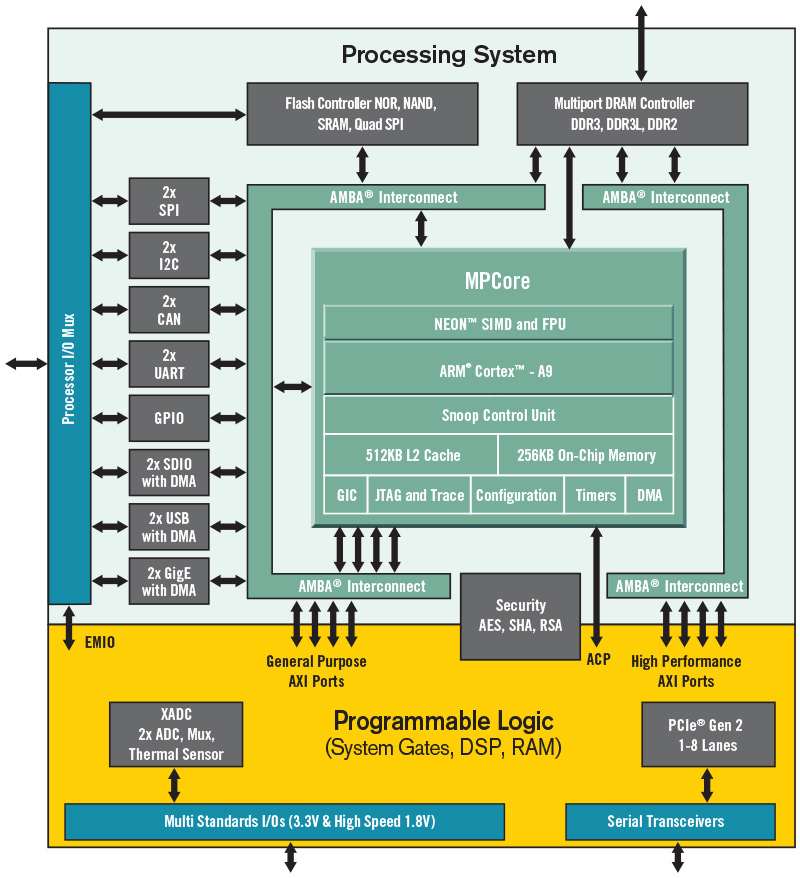
\includegraphics[width=0.6\textwidth]{images/zynq_arch.png}
\caption{Schema rappresentativo ZYNQ-7000\cite{Zynq-7000}}
\end{figure}\\
\section{Linguaggi di descrizione delle FPGA}
Come accennato nel capitolo, \ref{FPGA}, le FPGA vengono implementate tramite l'uso dei CAD da un progettista, risulta però utile avere conoscenze dei linguaggi di descrizione dell'hardware quali VHDL\cite{VHDL} e Verilog\cite{Verilog} . Entrambe le opzioni sono supportate da Vivado e sono valide al fine di descrivere il comporamento di un sistema digitale. Le principali differenze tra i due linguaggi sono le similitudini al linguaggio C, infatti il Verilog ricorda molto la struttura del linguaggio di programmazione, permettendo anche ad un utente novizio la comprensione e l'appoccio a questo tipo di linguaggio.\\
In generale entrambi i linguaggi sono intercambiabili per quanto rigurda la rappresentazione Register Transfer Level, ovvero la schematizzazione del sistema come un flusso di informazioni tra logica e registri. Inoltre entrambi condividono una struttura gerarchica, infatti è possibile tramite dei costrutti descrivere un sistema in maniera strutturale, tramite tre possibili approcci:
\begin{itemize}
    \item Comportamentale: Il programmatore ha il compito di descrivere il comportamento di un sistema tramite un algoritmo.
    \item Strutturale: Il programmatore descrive singolarmente ogni componente interno al sistema andando poi ad usare una combinazione per rappresentare il sistema.
    \item DataFlow: Il programmatore scrive il codice emulando il flusso di dati nel sistema.
\end{itemize}
Ogni approccio necessità la presenza di un Top Level Entity, ovvere il file principale che verrà sintetizzato e che ci permetterà di implementare l'FPGA, esso conterrà tutte le componenti, codici ed eventuali librerie o supporti.
\begin{figure}[h]
\centering
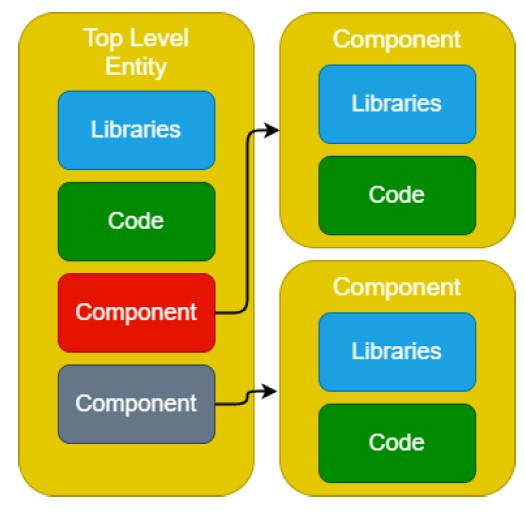
\includegraphics[width=0.3\textwidth]{images/VHFL.jpg}
\caption{Rappresentazione grafica di una Top Level Entity\cite{TesiMattia}}
\end{figure}\\
Una volta terminata la stesura del codice, ad oggi si usa solitamente per la creazione di IPCores custom, bisogna specificare le specifiche e limitazioni, i \textit{constraints}, che sono necessarie affinchè il sistema possa esser realizzato sulla scheda.
\section{Processo di Sviluppo FPGA}
Il processo di sviluppo non è riducibile alla scrittura del codice di definizione, come potrebbe avvenire per un arduino, ma necessità dei passaggi ulteriori dovuti all'architettura, infatti la presenza dell'interconnessione dei blocchi, i blocchi I/O necessariamente configurati e la programmable logic definita necessità la presenza di passaggi ulteriori.\\
L'evoluzione tecnologica ha portato ad avere grosse migliorie per quanto riguarda lo sviluppo, infatti ad oggi si parte dalla scrittura del codice\footnote{O generazione di esso tramite vivado}, passando il tutto ad un sistema di sintesi che ci permette di tradurre il tutto in una netlist, esso è un file che ci descrive tutte le interconnessioni logiche da effettuare tra i vari blocchi della scheda.\\

Per capire meglio il funzionamento dividiamo il processo in tre stadi:
Il primo stadio che prende il nome di \textit{Technology Mapping},effettua la generazione di un modello RTL (Register Transfer Level), questo stadio converte il codice di descrizione in dei blocchi più semplici, è importantissimo poichè bisogna garantire che le funzionalità descritte nel codice siano rispettate, esso si verifica tramite delle simulazioni. Alcuni blocchi di logica complessa vengono portati ad un livello composto tra gate logici e registri questo livello è detto Logic Gate Level.
\begin{figure}[h]
\centering
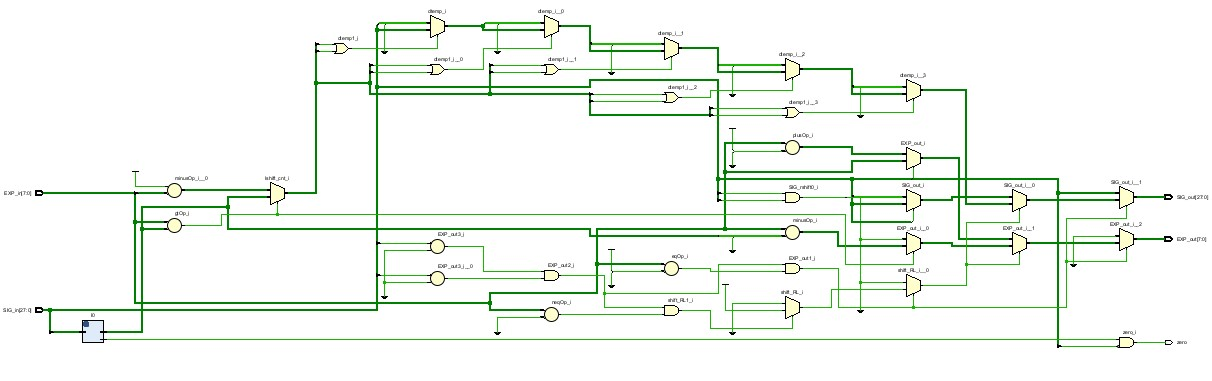
\includegraphics[width=0.8\textwidth]{images/RTL.jpg}
\caption{Rappresentazione grafica del Tecnology Mapping del FPGA in figura \ref{VIVADO1}}
\end{figure}\clearpage
Tutto questo processo viene ottimizzato come farebbe un compilatore, al fine di occupare meno spazio.\\
Una volta effettuato questo passaggio bisogna effettuare la collocazione degli elementi dell'FPGA, il procedimento prende il nome di \textit{Place \& Route} (\textit{PnR}), esso a sua volta è composto da tre sotto passaggi.\\
Il primo è il \textit{Packing}, esso analizza le primitive e le organizza in un cluster.\\
Il secondo è il \textit{Placing} prende in ingresso i cluster ed effettua la decisione di dove piazzare fisicamente i componenti sulla scheda permettendo cosi l'instradamento
\begin{figure}[h]
\centering
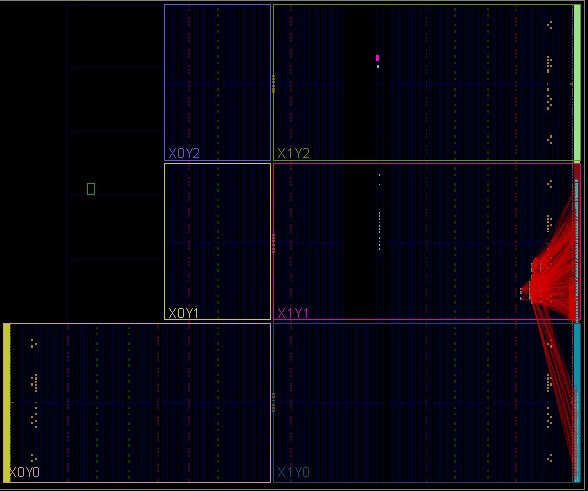
\includegraphics[width=0.4\textwidth]{images/Place.jpg}
\caption{Rappresentazione grafica del Placing del FPGA in figura \ref{VIVADO1}}
\end{figure}\\
In fine il \textit{Routing}, si occuperà di calcolare tutte le possibili connessioni scegliendo la migliore, in funzione del ritardo questo ovviamente rende il passaggio oneroso computazionalmente.
\begin{figure}[h]
\centering
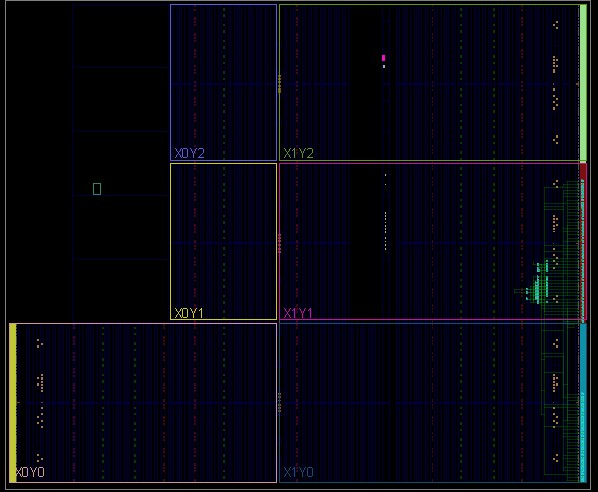
\includegraphics[width=0.4\textwidth]{images/Route.jpg}
\caption{Rappresentazione grafica del Routing del FPGA in figura \ref{VIVADO1}}
\end{figure}\\
Una volta terminati questi passaggi avremo a disposizione l'implementazione del FPGA, ma sarà necessario tradurre il tutto in un formato interpretabile al dispositivo, questo processo verrà ripreso anche in seguito. Questo passaggio di traduzione prende il nome di generazione del bitstream.
\begin{figure}[h]
\centering
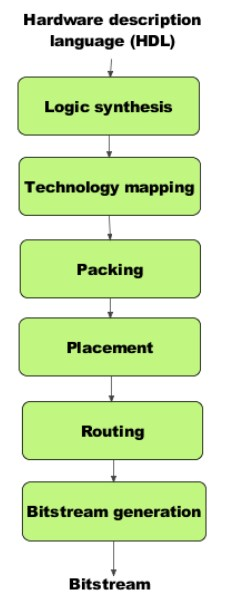
\includegraphics[width=0.2\textwidth]{images/Stack.jpg}
\caption{Stack per lo sviluppo di un FPGA}
\end{figure}\\
Questo tipo di sviluppo è il migliore nel nostro caso poichè non stiamo effettuando un High Level Synthesis (HLS), in quel caso esistono dei tools appositi.
\subsection{Sviluppo tramite Vivado}
Lo sviluppo tramite vivado è al quanto semplificato, poichè godendo di un interfaccia grafica permette l'implementazione di sistemi complessi anche non avendo alcuna conoscenza di VHDL o Verilog, si rimanda però all'appendice \ref{app:a} per maggiori chiarimenti su installazione ed inizio del primo progetto.
\section{Vitis}
Vitis è il Software Development Kit (SDK) fornito da Xilnix nella sua suite di prodotti, la sua installazione è contestuale a quella trattata in \ref{app:a}, tramite esso è possibile generare codice che in grado di esser eseguito sulla scheda, questo è possibile tramite le informazioni prese su vivado.\\
Sono presenti due possibilità di programmazione, standalone e linux, la prima applicazione permetterà l'esecuzione di codice C in modalità Bare-Metal\footnote{Livello di programmazione senza astrazioni, come il sistema operativo}, in questo modo potremmo usare delle librerie della Xilinix che contengono delle funzioni standard al fine di effettuare la comunicazione tra PS e PL. Successivamente tratteremo anche la comunicazione tra PS e PL su sistema linux. Questo tipo di programmazione è discussa approfonditamente \ref{Standalone}
\section{Petalinux}
È un tool della Xilinix che necessario qualora si volesse usare una distro Linux embedded su di una FPGA SoC xilinix, la sua installazione è trattata in \ref{petalinuxinst}. Petalinux offre una grossa flessibilità per la costruzione e compilazione di un kernel Linux, la sua flessibilità ci permette di escludere o includere moduli pre-esistenti oppure crearne uno noi secondo le nostre esigenze. Si basa fortemente sull'architettura e sull'esportazione che avviene da vivado al fine di costruire il device tree e tutti gli strumenti necessari al kernel.\\
Al fine di usufruire di petalinux vanno impostati i Jumpers della scheda MIO2-6 in configurazione  "00110", in questo modo potremmo usare il kernel che abbiamo creato e compilato\footnote{Che vedremo successivamente}, tramite la scheda SD che dovrà rispettare delle specifiche espresse in \ref{sd}.
\section{Bootgen}
Bootgen è un tool appartenente alla suite di sviluppo della Xilinix, il suo scopo è quello di generare i file binari e tutti gli artefatti necessari. La sua installazione verrà discussa in \ref{installazioneBoot}
Sfortunatamente questo tool è attualemente disponibile solo per architettura x86, quindi come tutti i tool presentati precedentemente non sarà possibile installarli sulla piattaforma da noi prescelta.\\